\documentclass[fr,license=none]{../../../eplnotes}

\usepackage{graphicx}
\usepackage{wrapfig}
\usepackage{subcaption}
\usepackage{array}
\usepackage{url}
\usepackage{mathrsfs}
\usepackage{textcomp}
\usepackage{upquote}
\usepackage{multirow}
\usepackage{fancyhdr}
\usepackage{ragged2e}
\usepackage{lscape}
\usepackage[export]{adjustbox}
\usepackage[squaren, Gray, cdot]{SIunits}
\usepackage{chngcntr}
\usepackage{comment}
\usepackage{float}
\usepackage[bottom]{footmisc}

\usepackage{tkz-euclide}
\usetkzobj{all}

\usepackage[lmargin=2cm,rmargin=7.5cm,marginparwidth=5cm,marginparsep=20pt]{geometry}

\usepackage{marginnote}
\usepackage{caption}

\newcommand\MarginFigBase[3]{%
\marginpar{#1
\captionof{figure}{#2}
\label{#3}}
}
\newcommand\MarginFig[4][width=\marginparwidth]{%
\marginpar{\includegraphics[#1]{#2}
\captionof{figure}{#3}
\label{#4}}
}

%\reversemarginpar

\usepackage{appendix}
\renewcommand{\appendixpagename}{Annexes}
\renewcommand{\appendixtocname}{Annexes}

\hypertitle{Description et analyse des mécanismes}{4}{MECA}{1210}
{Philippe Greiner\and Geoffroy Jacquet\and Martin Lefebvre\and Léa Paulus}
{Paul Fisette, Hervé Jeanmart et Benoît Herman}

Ce document contient toutes les démonstrations à connaître pour l'examen.
\section{Théorème d'Euler}
\textit{Tout déplacement d'un corps ayant un point fixe est une rotation autour d'un axe fixe passant par ce point.}

%\begin{wrapfigure}{R}{.3\linewidth}

%\vspace{-20pt}
%	\begin{center}
\MarginFig{Euler.png}{Illustatrion du théorème d'Euler}{Euler}
%	\end{center}
%	\vspace{-20pt}
	%\caption{Illustatrion du théorème d'Euler}
%	\vspace{-20pt}
	%\label{Euler}
%\end{wrapfigure}

En d'autres termes, il faut montrer qu'il existe un vecteur $\vec{e}$ pour lequel la rotation, représentée par la multiplication par une matrice $A$, n'aura pas d'influence. Montrant ainsi l'existence d'un axe fixe.

Ça revient à montrer qu'il existe un $e$ tel que:
$$e=Ae$$
qui est équivalent à
$$e-Ae=0$$
ce qui revient à
$$Ie-Ae=0$$
ou encore
$$(A-I)e=0$$
Comme $e$ est un vecteur non-nul, il faut que $(A-I)$ soit une matrice singulière. On sait que lorsqu'une matrice est singulière sont déterminant et nul, c'est à dire
$$\det (A-I)=0.$$
Or on sait également que les scalaires $\lambda$ telles que
$$\det (A-\lambda I)=0$$
sont les valeurs propres de $A$.
Il faudrait donc que $A$ ait 1 pour valeur propre.

$A$ étant une matrice $3 \times 3$\footnote{Parce qu'on est en 3D}, on a 3 valeurs propres.

La matrice $A$ étant orthogonale, on sait que $A^{-1} = A^T$. Or la matrice $A^T$ a les mêmes valeurs propres que $A$ et les valeurs propres de $A^{-1}$ sont l'opposé des valeurs propres de $A$.

Pour chaque valeur propre de $A$, son inverse est aussi valeur propre.
Le nombre de valeur propre étant impair, la seule solution c'est qu'une des valeurs propres soit 1, 1 étant égale à son inverse.


\section{Axe hélicoïdal instantané}
\MarginFig{helicoidal.png}{Illustration de l'axe hélicoïdale instantané}{helico}
On démontre que le vecteur vitesse angulaire $\vec{\omega}$ est parallèle à l'axe hélicoïdal instantané de rotation. Sur base de 2 points $P_1$ et $P_2$ appartenant à l'axe hélicoïdal, et non confondus, on écrit la vitesse d'un point A quelconque.
\begin{eqnarray}
\vec{v_A} &=& \vec{v_{P_1}} + \vec{\omega} \otimes \vec{P_1 A}
\\
\vec{v_A} &=& \vec{v_{P_2}} + \vec{\omega} \otimes \vec{P_2 A}
\end{eqnarray}

En égalant ces 2 résultats, et en tenant compte du fait que les points $P_1$ et $P_2$ se trouvent sur l'axe hélicoïdal, et ont donc la même vitesse car ils ne subissent qu'une translation et pas de rotation, on trouve que :
\begin{align*}
\vec{\omega} \otimes \vec{P_1 A} &= \vec{\omega} \otimes \vec{P_2 A}\\
\vec{\omega} \otimes (\vec{P_1 A} - \vec{P_2 A}) &= 0\\
\vec{\omega} \otimes (\vec{P_1 A} + \vec{A P_2}) &= 0\\
\vec{\omega} \otimes \vec{P_1 P_2} &= 0
\end{align*}

Cela démontre donc simplement que les vecteurs $\vec{\omega}$ et $\vec{P_1 P_2}$ sont parallèles.

\section{Détermination Analytique du c.i.r.}
\MarginFig{CIR.png}{Détermination analytique du \textit{c.i.r.}}{CIR}
On sait que pour un corps rigide :
\begin{align*}
\vec{v_B} &= \vec{v_A} + \vec{\omega} \otimes \vec{AB}\\
\vec{v_B} - \vec{v_A}  &= \vec{\omega} \otimes \vec{AB}\\
\vec{AB} \otimes (\vec{v_B} - \vec{v_A})  &= \vec{AB} \otimes (\vec{\omega} \otimes \vec{AB})
\end{align*}

En utilisant la propriété du produit vectoriel $\vec{a} \otimes \vec{b} = -\vec{b} \otimes \vec{a}$, on trouve que :
$$\vec{AB} \otimes (\vec{v_B} - \vec{v_A})  = -(\vec{\omega} \otimes \vec{AB}) \otimes \vec{AB}$$

En appliquant le fait que $\vec{u} \otimes (\vec{v} \otimes \vec{w}) = \vec{v}(\vec{u} \cdot \vec{w}) - \vec{w}(\vec{v} \cdot \vec{u})$, on obtient alors :
$$\vec{AB} \otimes (\vec{v_B} - \vec{v_A})  = -\vec{AB}(\vec{\omega} \cdot \vec{AB}) +\vec{\omega} \| \vec{AB} \|^2 $$

En tenant compte du fait que $\vec{\omega} \cdot \vec{AB} = 0$, le vecteur $\vec{\omega}$ est donné par :
$$\vec{\omega} = \frac{\vec{AB} \otimes (\vec{v_B} - \vec{v_A})}{\| \vec{AB} \|^2 }$$

On peut maintenant calculer la position du CIR.
\begin{align*}
\vec{v_A} &= \vec{\omega} \otimes \vec{IA} = \vec{AI} \otimes \vec{\omega}\\
\vec{\omega} \otimes \vec{v_A} &= \vec{\omega} \otimes (\vec{AI} \otimes \vec{\omega})\\
\vec{\omega} \otimes \vec{v_A} &= -(\vec{AI} \otimes \vec{\omega}) \otimes \vec{\omega}\\
\vec{\omega} \otimes \vec{v_A} &= -\vec{\omega}(\vec{AI} \cdot \vec{\omega}) + \vec{AI}\|\vec{\omega}\|^2\\
\vec{AI} &= \frac{\vec{\omega} \otimes \vec{v_A}}{\|\vec{\omega}\|^2}
\end{align*}

\section{Calcul des base et roulante pour une échelle}
\MarginFig{baseroulante2.png}{Détermination analytique de la base et de la roulante}{baseroul}


Dans le cas de la base, on constate que le CIR correspond au sommet (avec l'angle droit) du triangle rectangle dont l'hypoténuse est définie par l'échelle de longueur L. Le lieu géométrique est donc simplement un cercle dont l'équation est donnée par :
$$X^2 + Y^2 = L^2$$

Dans le cas de la roulante, on exprime les coordonnées X et Y en fonction de l'angle $\alpha$ formé par l'axe vertical et l'échelle, et des coordonnées x et y dans le repère solidaire de l'échelle.
\begin{eqnarray}
X &=& L \cdot \sin\alpha + x \cdot \cos\alpha - y \cdot \sin\alpha
\\
Y &=& x \cdot \sin\alpha + y \cdot \cos\alpha
\end{eqnarray}

On dérive ensuite ces 2 équations par rapport au temps pour calculer les vitesses en x et y, et on les égale à 0, car le CIR est le point géométrique correspondant au point matériel à vitesse nulle.
\begin{eqnarray}
\dot{X} &=& \dot{\alpha} \cdot (L \cdot \cos\alpha - x \cdot \sin\alpha - y \cdot \cos\alpha)
\\
\dot{Y} &=& \dot{\alpha} \cdot (x \cdot \cos\alpha - y \cdot \sin\alpha)
\end{eqnarray}

En simplifiant les $\dot{\alpha}$ des 2 équations, et en multiliant la première par $x \cdot \sin\alpha$ et la seconde par $x \cdot \cos\alpha$, puis en soustrayant la première à la seconde, on obtient :
$$ x^2 \cdot \sin^2 \alpha +  x^2 \cdot \cos^2 \alpha = Lx \cdot \cos \alpha \cdot \sin \alpha$$
En transformant $\sin \alpha \cdot \cos \alpha$ en $\frac{\sin(2 \alpha)}{2}$, on obtient :
$$x = \frac{L \cdot \sin(2 \alpha)}{2}$$

\noindent
En remplaçant $x$ par sa valeur dans l'équation $y = \frac{x \cdot \cos\alpha}{\sin \alpha}$, on trouve que :
$$y = L \cdot \cos^2 \alpha$$
En transformant $\cos^2 \alpha$ en $\frac{1+\cos(2 \alpha)}{2}$, on obtient :
$$y - \frac{L}{2} = \frac{L \cdot \cos(2 \alpha)}{2}$$

\noindent
Sur base des valeurs trouvées pour x et y, on peut exprimer l'équation de la roulante dans la base solidaire de l'échelle.
$$x^2 + (y-\frac{L}{2})^2 = (\frac{L}{2})^2$$
\section{Vitesse et accélération d'une bielle}
\MarginFigBase{
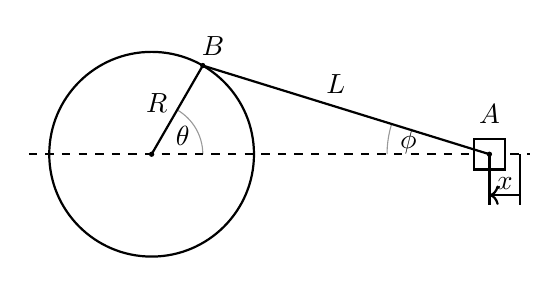
\begin{tikzpicture}[x=1.3cm,y=1.3cm]
  \coordinate (C) at (0,0);
  \coordinate (A) at (3.3,0);
  \coordinate (B) at (1/2,1.732/2);
  \draw[dashed, thick] (-1.2,0) to (3.7,0);
  \draw[thick] (0,0) circle (1);
  \tkzMarkAngle[fill= orange,size=1,opacity=.4](B,A,C)
  \tkzLabelAngle[pos = 0.8](B,A,C){$\phi$}
  \fill[white] (3.15,-0.15) rectangle (3.45,0.15);
  \draw[thick] (3.15,-0.15) rectangle (3.45,0.15);
  \draw[thick] (0,0) to (1/2,1.732/2) to (3.3,0);
  \node[left] at  (1/4, 0.5) {$R$};
  \node[above] at  (1.8, 0.5) {$L$};
  \node[above] at  (3.3, .2) {$A$};
  \filldraw (0, 0) circle (.02);
  \filldraw (1/2, 1.732/2) circle (.02);
  \filldraw (3.3, 0) circle (.02);
  \node[above] at  (0.6, 1.732/2) {$B$};
  \draw[thick] (3.3,0) to (3.3,-.5);
  \draw[thick] (3.6,0) to (3.6,-.5);
  \draw[thick,->] (3.6,-.4) to (3.3,-.4);
  \node[above] at (3.45, -.44) {$x$};
  \tkzMarkAngle[fill= orange,size=.5,%
  opacity=.4](A,C,B)
  \tkzLabelAngle[pos = 0.35](A,C,B){$\theta$}
\end{tikzpicture}}{Bielle-manivelle}{bielleman}

Regardons le déplacement du point $A$ sur la figure~\ref{bielleman}, on peut le définir comme ceci:
$$x_A= R + L - (R \cos \theta + L \cos \phi),$$
Avec $R \sin \theta = L \sin \phi$.
\begin{align*}
x_A &= R + L - (R \cos \theta + L \cos \phi)\\
&= R( 1 -\cos \theta + L(1-\cos \phi)
\end{align*}
Où $$1-\cos \phi = 1 - \sqrt{1- \dfrac{R^2}{L^2}\sin ^2 \theta}$$
Avec Taylor d'ordre 1, on a:
$$\sqrt{1-x}\simeq 1 -\dfrac{x}{2}.$$
Ce qui nous donne:
$$\sqrt{1-\dfrac{R^2}{L^2}\sin ^2 \theta}\simeq 1 -\dfrac{R^2}{2 L^2}\sin ^2 \theta.$$
On obtient donc,
\begin{align*}
x_A &= R(1 - \cos \theta) + L \left( 1 - \left( 1 - \dfrac{R^2}{2 L^2}\sin ^2 \theta \right) \right)\\
&= R(1 - \cos \theta) + \dfrac{R^2}{2 L}\sin ^2 \theta.
\end{align*}


Pour la vitesse du point $A$ on a:
\begin{align*}
v&= \dot{x} \\
&= R \dot{\theta} \sin \theta \\
&= R \omega \sin \theta.
\end{align*}
Pour l'accélération du point $A$ on a:
\begin{align*}
a&= \dot{v} \\
&= R\omega \dot{\theta} \cos \theta \\
&= R \omega ^2 \cos \theta.
\end{align*}
\section{Guidage elliptique-orthogonal}
\MarginFig{elliptique.png}{Détermination analytique du guidage elliptique}{elli}

Montrons que pour tout point de la bielle la trajectoire est elliptique, représenté sur la figure~\ref{elli}:
$\forall D \in AB,$ on a:
\begin{equation}\label{Xd}
\frac{X_D}{BD}=\frac{OA}{L}
\end{equation}
\begin{equation}\label{Yd}
\frac{Y_D}{AD}=\frac{OB}{L}
\end{equation}
En prenant $\ref{Xd}^2 + \ref{Yd}^2$, on obtient:
\begin{align*}
\frac{X_D^2}{BD^2}+\frac{Y_D^2}{AD^2}&=\frac{OA^2}{L^2}+\frac{OB^2}{L^2}\\
&=1
\end{align*}
Ce qui nous donne une ellipse de demis-axes $BD$ et $AD$ dont le point milieu $E$ décrit un cercle.
\section{Joint de Cardan}
\begin{figure}[h!]
\centering
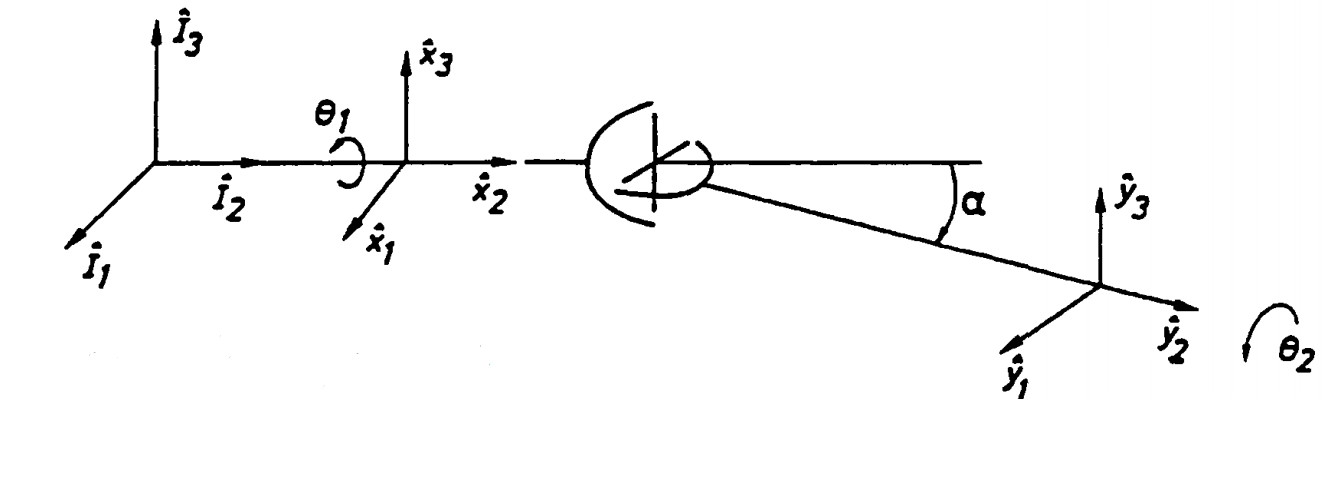
\includegraphics[width=.8\linewidth]{cardan}
\caption{Joint de Cardan}
\label{jointDeCard}
\end{figure}
Soient $\theta_1$ l'angle d'entrée, $\omega_1$ la vitesse angulaire d'entrée, $\theta_2$ l'angle de sortie et $\omega_2$ la vitesse angulaire de sortie, représentés à la figure~\ref{jointDeCard}. Les repères $[\hat{I}]$, $[\hat{x}]$ lié à l'arbre 1 et $[\hat{y}]$ lié à l'arbre 2.

\paragraph{Relations entre bases}
On a les relations suivantes: \\ \newline
$ [\hat{x}] = A^{(2)}(\theta_1)\cdot [\hat{I}] = \begin{pmatrix} \cos\theta_1 & 0 & -\sin\theta_1 \\ 0 & 1 & 0 \\ \sin\theta_1 & 0 & \cos\theta_1 \end{pmatrix} \begin{pmatrix} \hat{I_1}\\ \hat{I_2} \\ \hat{I_3} \end{pmatrix}$ \\
$ [\hat{y}] = A^{(2)}(\theta_2)\cdot A^{(3)}(-\alpha)\cdot [\hat{I}] = \begin{pmatrix} \cos\theta_2\cdot  \cos\alpha & -\cos\theta_2\cdot  \sin\alpha & -\sin\theta_2 \\ \sin\alpha & \cos\alpha & 0 \\ \sin\theta_2\cdot  \cos\alpha & -\sin\theta_2\cdot  \sin\alpha & \cos\theta_2 \end{pmatrix} \begin{pmatrix} \hat{I_1}\\ \hat{I_2} \\ \hat{I_3} \end{pmatrix}$
\paragraph{Contrainte dûe au croisillon}
Le croisillon introduit la contrainte suivante : $\hat{y_1}\perp \hat{x_3}$, donc $\hat{y_1}\cdot \hat{x_3} = 0$.\\
En effectuant ce produit scalaire, on obtient $$\sin\theta_1\cdot \cos\theta_2\cdot \cos\alpha - \cos\theta_1\cdot \sin\theta_2 = 0.$$
On divise cette relation par $\cos\theta_1\cdot \cos\theta_2$ pour obtenir: \begin{equation}\label{tg} tg\theta_2 = tg\theta_1\cdot \cos\alpha \end{equation}
On dérive\footnote{On se souviendra que $(tg\ \alpha)^\prime = \frac{1}{\cos^2\alpha}$, et $\dot{\theta_i} = \omega_i$} par rapport au temps, ce qui donne :
$$\frac{\omega_2}{\omega_1} = \cos\alpha\cdot\frac{\cos^2\theta_2}{\cos^2\theta_1}$$
En utilisant succesivement $\cos^2\theta_2 = \frac{1}{1 + tg^2\theta_2}$ puis la relation (\ref{tg}), on obtient le résultat final (en remplaçant $\cos^2\alpha$ par $1 - \sin^2\alpha$) :
$$\boxed{ \frac{\omega_2}{\omega_1} = \frac{\cos\alpha}{1 - \sin^2\theta_1\cdot \sin^2\alpha}}$$
Notons que le maximum se situe en $\frac{1}{\cos\alpha}$ (quand $\theta_1 = \frac{\pi}{2}$) et le minimum en $\cos\alpha$ (pour $\theta_1 = 0$).

\section{Formule de Willis}
\MarginFig{willis.png}{Formule de Willis}{Willis}
Les deux roues sont en RSG. Pour imposer cette condition, il suffit d'écrire la vitesse du point matériel de contact de chacune des roues, puis d'égaler ces vitesses. Pour imposer le contact au PMC, on a $\vec{R_1} + \vec{r_1} = \vec{R_2} + \vec{r_2}$, c'est-à-dire $ \vec{R_1} - \vec{R_2} = \vec{r_2} - \vec{r_1}$. \\ On a donc, avec $\Omega$ la vitesse de rotation du châssis: \begin{equation*}\begin{split}
\vec{v_1} = \dot{\vec{R_1}} + \dot{\vec{r_1}} = \vec{\Omega} \times \vec{R_1} + \vec{\omega_1} \times \vec{r_1}\\
\vec{v_2} = \dot{\vec{R_2}} + \dot{\vec{r_2}} = \vec{\Omega} \times \vec{R_2} + \vec{\omega_2} \times \vec{r_2}
\end{split} \end{equation*}
En posant $\vec{v_1} - \vec{v_2} = 0$ on obtient: $$\vec{\Omega} \times (\vec{R_1} - \vec{R_2}) + \vec{\omega_1} \times \vec{r_1} - \vec{\omega_2} \times \vec{r_2} = 0$$
En remplaçant $\vec{R_1} - \vec{R_2}$ par $\vec{r_2} - \vec{r_1}$, on a (en regroupant les termes): $$ (\vec{\omega_1} - \vec{\Omega}) \times \vec{r_1} = (\vec{\omega_2} - \vec{\Omega}) \times \vec{r_2}$$
Ce qui donne la formule de Willis: $\boxed{\frac{\omega_2 - \Omega}{\omega_1 - \Omega} = \pm |\frac{r_1}{r_2}|}$, le signe négatif correspondant à un roulement extérieur ($\vec{r_1}$ et $\vec{r_2}$ sont de directions opposées) et le signe positif à un roulement intérieur.

\paragraph{Trains de roulement} Pour généraliser la formule à un train de roulement à n roues, on utilisera simplement le fait que $$\frac{\omega_n - \Omega}{\omega_1 - \Omega} = \frac{\omega_n - \Omega}{\omega_{n-1} - \Omega} \cdot \frac{\omega_{n-1} - \Omega}{\cdots} (\cdots) \frac{\cdots}{\omega_1 - \Omega}$$ pour appliquer n fois la formule de Willis.

\section{Condition d'engrènement}
\MarginFig{engrenement.png}{Condition d'engrènement}{engrennement}

Soient deux profils articulés, $M_1$ et $M_2$. Pour qu'il n'y ait pas pénétration, il faut que leurs vitesses normales au point de contact soient égales. Cette condition donne donc $$ (\vec{\omega_1}\times \vec{O_1M})\cdot\vec{MP} = (\vec{\omega_2}\times \vec{O_2M})\cdot \vec{MP}$$
Comme $\vec{O_1M} = \vec{O_1P} + \vec{PM} \text{ et } \vec{O_2M} = \vec{O_2P} + \vec{PM}$, cela équivaut\footnote{puisque $(\vec{u}\times\vec{v})\cdot\vec{v} = 0$} à $$ (\vec{\omega_1}\times \vec{O_1P})\cdot\vec{MP} = (\vec{\omega_2}\times \vec{O_2P})\cdot \vec{MP}.$$
Avec $\vec{\omega_i} = \omega_i.\hat{I_3}$ et $\vec{O_iP} = O_iP.\hat{I_2}$, on a alors:
\begin{align*}
\omega_1\ O_1P(\hat{I_1}\cdot \vec{MP}) = \omega_2\ O_2P(\hat{I_1}\cdot \vec{MP}) \end{align*}
et donc on obtient
\begin{align*}
\omega_1\ O_1P = \omega_2\ O_2P
\end{align*}
où $O_1P$ est négatif (voir dessin).

Le rapport de transmission $\frac{\omega_1}{\omega_2} = -\frac{|O_2P|}{|O_1P|}$ dépend de P: il faut donc P fixe pour avoir un rapport de transmission constant. En introduisant $R_1 = |O_1P|$ et $R_2 = |O_2P|$, on définit donc les rayons des cercles primitifs.
\paragraph{Condition fondamentale d'engrènement} Les profils en prise sont tels qu'\textbf{à tout moment}, la normale commune au point de contact (M) passe par un point P \textbf{fixe}, point de tangence des cercles primitifs.

\section{Vitesse de glissement au contact}
\noindent On a $ -\frac{\omega_1}{\omega_2} = \frac{R_2}{R_1}.$
On calcule les composantes tangentielles des vitesses au point de contact, et on les soustrait:
\begin{align*}
\vec{v_g} &= ((\vec{\omega_2}\times \vec{O_2M}) - (\vec{\omega_1}\times \vec{O_1M}))\cdot \hat{t}\\
&= ((\vec{\omega_2}\times (\vec{O_2P} + \vec{PM})) - (\vec{\omega_1}\times (\vec{O_1P} + \vec{PM})))\cdot \hat{t}\\
&= ((\vec{\omega_2}\times \vec{PM}) - (\vec{\omega_1}\times \vec{PM}))\cdot \hat{t}\footnotemark
\end{align*}
\footnotetext{Où on a utilisé la condition d'engrènement pour éliminer $\vec{\omega_2}\times \vec{O_2P} - \vec{\omega_1}\times \vec{O_1P}$, vecteurs opposés d'amplitude égale.}
\noindent On obtient donc la vitesse de glissement, $$\boxed{|\vec{v_g}| = |(|\omega_1|\pm|\omega_2|)|PM||.}$$
Le signe négatif, d'application dans le cas de roulement \textbf{intérieur}, est dû au fait que $\vec{\omega_1}$ et $\vec{\omega_2}$ ont alors la même direction. Physiquement, cela correspond à la réalité: un roulement intérieur entraîne un glissement moindre.

\section{Résistance au roulement}
On a $ I=\frac{Mr^2}{2},\quad \dot{R} = r\dot{\Theta}\ \text{(RSG)},\quad \omega = \dot{\Theta}.$ Soit $a$, la distance (due à a déformation de la roue) entre l'application de $\vec{T}$ et de $\vec{N}$.
On commence par écrire les équations de Newton:
\begin{align*}
\hat{I_1}: &\qquad T = M\ddot{R} \\
\hat{I_3}: &\qquad P = N
\end{align*}
\MarginFig{coupleroulement.png}{Couple de roulement}{coupleroulement}
\MarginFig{roulement.png}{Roulement}{roulement}

On fait maintenant la somme des couples par rapport au centre de la roue, ce qui donne successivement :
\begin{align*}
r\hat{I_3}\times T\hat{I_1} + (-a)\hat{I_1}\times N\hat{I_3} &= \frac{Mr^2}{2}\cdot \dot{\omega}\hat{I_2}\\
-rT-aN &= \frac{Mr^2}{2}\cdot \dot{\omega}\\
T &= -\frac{aN}{r} - \underbrace{\frac{Mr}{2}\ddot{\Theta}}_{T/2}\\
%\frac{3}{2}T &= -\frac{aN}{r}\\
T &= -\frac{2}{3}\frac{aP}{r}
\end{align*}

On a trouvé la force tangentielle en application, il reste maintenant à montrer que le couple engendré par $\vec{F} = \vec{T} + \vec{N}$ est un couple retardateur.
On se réfère à la figure ci-contre pour le nom des variables. On a $tg\ \alpha = \frac{a}{r}.$ On calcule ensuite: $tg\ \beta = |\frac{T}{N}| = \frac{2}{3}\frac{a}{r}=\frac{2}{3}tg\ \alpha.$ On a donc forcément $\beta < \alpha$, donc le couple engendré par $\vec{F}$ passe devant le centre de la roue, et est un couple retardateur.


\section{Démarrage sur plan incliné}
\subsection{Force parallèle au plan incliné}

\MarginFig{fext.png}{Effort $F_{ext}$ parallèle au plan incliné.}{planincli}
On a $N = P\cdot \cos\ \alpha$ ainsi que $T = N\cdot tg\ \phi_0$. On va maintenant faire la somme des forces, pour connaître la force permettant 'tout juste' de démarrer vers le haut ($\vec{F^\prime}_{ext}$) ainsi que celle permettant tout juste de démarrer vers le bas ($\vec{F}^{\prime\prime}_{ext}$). On a donc ($+$ pour $\vec{F^\prime}_{ext}$):
\begin{align*}
F^{\prime(\prime)}_{ext} &= P\cdot \sin\ \alpha \pm T\qquad\qquad [\hat{I_1}]\\
&= P\cdot \sin\ \alpha \pm N\cdot tg\ \phi_0\\
&= P\cdot \sin\ \alpha \pm P\cdot \cos\ \alpha\cdot  tg\ \phi_0\\
F^{\prime(\prime)}_{ext}\cdot \cos\ \phi_0 &= P\cdot \sin\ \alpha\cdot \cos\ \phi_0 \pm P\cdot \cos\ \alpha\cdot \sin\ \phi_0
\end{align*}
En utilisant maintenant la formule pour $\sin(a\pm b)$, on obtient $\boxed{F^{\prime(\prime)}_{ext} = P\cdot \frac{\sin(\alpha\pm \phi_0)}{\cos\ \phi_0}}$.

\subsection{Force horizontale}
La figure de cette démonstration est identique à la précédente, avec $H_{ext}$ horizontale. En appliquant cet effort horizontal, on a (pour $H^{\prime\prime}_{ext}$, il suffit de commencer avec $-T\cos\ \alpha$):
$$H^{\prime}_{ext} = N\cdot \sin\ \alpha \pm T\cdot \cos\ \alpha$$
On sait que $N = H^\prime_{ext}\cdot \sin\ \alpha + P\cdot \cos\ \alpha$, et $T \stackrel{\triangle}{=}N\cdot tg\ \phi_0$. En remplaçant cela dans la formule ci-dessus, on obtient
\begin{align*}
H^{\prime}_{ext} &= H^\prime_{ext}\cdot \sin^2\alpha + P\cdot \sin\ \alpha\cdot  \cos\ \alpha\\
& \quad {} + (H^\prime_{ext}\cdot \sin\ \alpha + P\cdot \cos\ \alpha)\cdot \cos\ \alpha\cdot  tg\ \phi_0\\
H^{\prime}_{ext}\cdot (\underbrace{1 - \sin^2\alpha}_{\cos^2\alpha} - \sin\ \alpha\cdot  \cos\ \alpha\cdot  tg\ \phi_0) &= P\cdot \cos\ \alpha\cdot  (\sin\ \alpha + \cos\ \alpha\cdot  tg\ \phi_0)\\
H^{\prime}_{ext} &= P\cdot \frac{\sin\ \alpha + \cos\ \alpha\cdot  tg\ \phi_0}{\cos\ \alpha - \sin\ \alpha\cdot  tg\ \phi_0}\cdot \frac{\cos\phi_0}{\cos\phi_0}
\end{align*}
En employant les formules pour $\sin(a + b)$ et $\cos(a+b)$, on obtient $\boxed{H^{\prime}_{ext} = P\cdot \frac{\sin(\alpha+\phi_0)}{\cos(\alpha+\phi_0)} = P\cdot tg(\alpha + \phi_0).}$

\section{Embrayage à disque: couple maximal}
\subsection{Hypothèse de pression uniforme}
Sous l'hypothèse de pression uniforme, on a $p = \frac{nF}{\pi(r^2_2 - r^2_1)}$. La pression est due à $n$ boulons de serrage $F$.
Le couple maximal transmissible est alors $$M_{max} = \int^{r_2}_{r_1}2\pi r\cdot fpr\ dr = \frac{2}{3}fnF\frac{r^3_2 - r^3_1}{r^2_2 - r^2_1}.$$
Cette relation est la même que celle des plateaux d'accouplement.
\subsection{Hypothèse d'usure uniforme}
L'hypothèse d'usure uniforme implique deux choses:
\begin{itemize}
\item Vitesse d'usure $\propto$ Puissance dissipée $$\dot{u} = fp\omega r$$
\item Usure uniforme $\implies$ $\dot{u}, f$ et $\omega$ constants $$\implies pr = C$$
\end{itemize}
On cherche d'abord à trouver la constante C. On a donc, avec $P = nF$:
$$P = \int^{r_2}_{r_1}p\cdot2\pi rdr = 2\pi\int^{r_2}_{r_1}C dr = 2\pi C(r_2 - r_1) \iff C = \frac{P}{2\pi(r_2-r_1)}.$$
On calcule maintenant le moment maximal: $$M_{max} = \int^{r_2}_{r_1}fpr\cdot2\pi rdr = 2\pi fC\frac{r^2_2-r^2_1}{2} = fP\frac{r_1 + r_2}{2}.$$

\section{Tension sur une courroie}

On cherche à trouver la relation entre la tension d'entrée et de sortie sur une courroie. Avec $p\ [N/m]$ la force par unité de longueur, on peut écrire l'équilibre des forces selon l'axe de symétrie:
\begin{align}
prd\theta - t\cdot \sin\frac{d\theta}{2} - (t + dt)\cdot \sin\frac{d\theta}{2} &= 0 \nonumber\\
 \text{en négligeant les termes du second ordre}&\Updownarrow \text{et avec $\sin\frac{d\theta}{2}\approx \frac{d\theta}{2}$}\nonumber \\
prd\theta - td\theta &= 0 \nonumber \\
t &= pr \label{courroie}
\end{align}
\MarginFig{courroie.png}{Tension dans une courroie}{courroie}

On fait maintenant l'équilibre suivant la tangente à la courroie, ce qui donne
\begin{align}
(t+dt)\cos\frac{d\theta}{2} - fprd\theta - t\cos\frac{d\theta}{2} &= 0\nonumber\\
\text{en négligeant le second ordre } &\Updownarrow \text{ et avec $\cos\frac{d\theta}{2}\approx1$}\nonumber\\
dt &= fprd\theta\stackrel{(\ref{courroie})}{=}ftd\theta\nonumber\\
\int_{T_0}^{t}\frac{dt}{t} &= \int_{\theta_0}^{\theta}fd\theta\nonumber\\
ln\frac{t}{T_0} &= f\cdot(\theta-\theta_0)\nonumber
\end{align}
On a donc, pour $t = T_1$ et $\theta=\theta_1$, $\boxed{T_1 = T_0\cdot e^{f\alpha}}$.

\section{Limite d'adhérence d'une courroie}
On se réfère au même schéma que pour la section précédente, lors du calcul de la tension sur la courroie. Pour calculer la limite d'adhérence de la courroie, on calcule l'équilibre quasi-statique selon l'axe de symétrie, en tenant compte de l'accélération centripète ($= -\omega^2r = -\frac{v^2}{r}$) de la courroie. Avec $\mu [kg/m]$, on a alors:
\begin{align}
prd\theta - t\cdot \sin\frac{d\theta}{2} - (t + dt)\cdot \sin\frac{d\theta}{2} &= -\mu rd\theta\cdot \frac{v^2}{r}\nonumber\\
prd\theta - t\cdot d\theta &= -\mu v^2d\theta\nonumber\\
pr &= t - T_c\text{\qquad \qquad avec $T_c = \mu v^2$ la tension centripète.} \label{tc}
\end{align}

On calcule maintenant l'équilibre selon la tangente, avec $F_{frottement}\le fprd\theta$. En effectuant les mêmes approximations que pour le calcul de la tension, on a:
\begin{align*}
dt &\le fprd\theta\\
dt &\stackrel{(\ref{tc})}{\le} f\cdot (t-T_c)\cdot d\theta\\
\int^{T_1}_{T_0}\frac{dt}{t-T_c} &\le \int^{\theta_1}_{\theta_0}fd\theta\\
\frac{T_1-T_c}{T_0-T_c} &\le e^{f\alpha}
\end{align*}
Pour obtenir la limite d'adhérence, on remplace le $\le$ par une égalité, ce qui donne $\boxed{T_1 = T_0\cdot e^{f\alpha} - T_c\cdot (e^{f\alpha}-1)}$.

\appendix
\appendixpage
\addappheadtotoc
\section{Calcul de l'angle de rendement maximal pour une vis sans fin}

Le rendement du mécanisme à vis sans fin est donné par :
$$\eta = \frac{\tan(\alpha)}{\tan (\alpha + \phi_0)}$$

On calcule la dérivée $\fdif{\eta}{\alpha}$ et on l'égalise à 0.
$$\fdif{\eta}{\alpha} = \frac{\frac{1}{\cos^2 \alpha} \cdot \tan (\alpha + \phi_0) - \tan( \alpha) \cdot \frac{1}{\cos^2 (\alpha + \phi_0)}}{\tan^2(\alpha + \phi_0)} = 0$$
$$\frac{\cos(\alpha + \phi_0)\cdot \sin(\alpha + \phi_0) - \cos(\alpha) \cdot \sin(\alpha)}{\sin^2(\alpha + \phi_0) \cdot \cos^2(\alpha)} = 0$$
$$\cos(\alpha + \phi_0)\cdot \sin(\alpha + \phi_0) = \cos(\alpha) \cdot \sin(\alpha)$$

En utilisant la formule $\sin(a)\cos(a) = \frac{\sin(2a)}{2}$, on obtient :

$$\sin(2 \cdot (\alpha + \phi_0)) = \sin(2 \cdot \alpha)$$

La résolution de cette équation trigonométrique conduit à :
\begin{align*}
2 \alpha + 2 \phi_0 &= \pi - 2\alpha\\
4 \alpha  &= \pi - 2\phi_0\\
\alpha &= \frac{\pi}{4} - \frac{\phi_0}{2}
\end{align*}

\end{document}
